% \documentclass[12pt,aspectratio=169]{beamer}
\documentclass[10pt]{beamer}

\mode<presentation>

% import packages
\usepackage{booktabs}
\usepackage{tabularx}
\usepackage{graphicx}
\usepackage{caption}
\usepackage{pdfrender}
\usepackage{setspace}
\usepackage{array}
\usepackage{minted}
\usepackage{listings}
\usepackage{xcolor}
\usepackage{tikz}
\usepackage{tikz-qtree}
\usetikzlibrary{arrows,shapes}

\newminted{python}{fontsize=\scriptsize, 
                   linenos,
                   numbersep=8pt,
                   gobble=4,
                   frame=lines,
                   bgcolor=bg,
                   framesep=3mm} 

% set up fonts
\usepackage[bitstream-charter]{mathdesign}
\usepackage[sfdefault,lining]{FiraSans}
\usepackage{FiraMono}
\usepackage[T1]{fontenc}
\usepackage{parnotes}

% define colours
\definecolor{MatiesMaroon}{RGB}{96,34,59}
\definecolor{MatiesGold}{RGB}{150,113,64}
\definecolor{MatiesYellow}{RGB}{240,179,54}
\definecolor{MatiesScienceRed}{RGB}{180,22,44}
\definecolor{MatiesAgriScienceGreen}{RGB}{61,138,26}
\definecolor{MatiesEducationBlue}{RGB}{34,61,113}
\definecolor{MatiesLightGrey}{HTML}{FAFAFA}
\definecolor{MatiesDarkGrey}{HTML}{212121}

\definecolor{DarkPurple}{HTML}{871f78}
\definecolor{darkgray}{rgb}{.4,.4,.4}
\definecolor{purple}{rgb}{0.65, 0.12, 0.82}

% colours for listings
\definecolor{keyword}{HTML}{2771a3}
\definecolor{pattern}{HTML}{b53c2f}
\definecolor{string}{HTML}{be681c}
\definecolor{relation}{HTML}{7e4894}
\definecolor{variable}{HTML}{107762}
\definecolor{comment}{HTML}{8d9094}

\lstset{
	numbers=none,
	stepnumber=1,
	numbersep=5pt,
	basicstyle=\small\ttfamily,
	keywordstyle=\color{keyword}\bfseries\ttfamily,
	commentstyle=\color{comment}\ttfamily,
	stringstyle=\color{string}\ttfamily,
	identifierstyle=\color{black},
	showstringspaces=false,
	aboveskip=3pt,
	belowskip=3pt,
	columns=flexible,
	keepspaces=true,
	breaklines=true,	
	captionpos=b,
	tabsize=2,
	frame=none
}

% Listing rules for Cypher

\lstdefinelanguage{cypher}
{
    morekeywords={
		MATCH, OPTIONAL, WHERE, NOT, AND, OR, XOR, RETURN, DISTINCT, ORDER, BY, ASC, ASCENDING, DESC, DESCENDING, UNWIND, AS, UNION, WITH, ALL, CREATE, DELETE, DETACH, REMOVE, SET, MERGE, SET, SKIP, LIMIT, IN, CASE, WHEN, THEN, ELSE, END, INDEX, DROP, UNIQUE, CONSTRAINT, EXPLAIN, PROFILE, START, CALL
	},
    ndkeywords={pageRank, iterate},
    keywordstyle={\color{keyword}\bfseries},
    ndkeywordstyle= {\color{relation}},
    sensitive=true
}

% Listing rules for Gremlin

\lstdefinelanguage{gremlin}
{
    keywordstyle = {\color{keyword}},
    morekeywords = {
        has, outE, order, by, desc, asc, inV, select, circle, gt, lt, leq, as, geoWithin, hasLabel, out, except, V, where, values, neq, eq, valueMap, limit, in, dedup, fold, unfold, inE, between, union, filter, get, value, atZone, of, getMonthValue, toLocalDate
    },
    ndkeywords={Geoshape, ZoneId},
    ndkeywordstyle= {\color{relation}},
    sensitive=true,
    morestring=*[d]{"},
}

% Listing rules for GSQL

\lstdefinelanguage{gsql}
{
	morekeywords={
		CREATE, QUERY, FOR, GRAPH, SELECT, FROM, WHERE, PRINT, ACCUM, INTERSECT, TYPEDEF, LIMIT, DO, FOREACH, RANGE, DO, IN, END, YEAR, MONTH
	},
	keywordstyle=\color{keyword}\bfseries,
	ndkeywords={SetAccum, ListAccum, HeapAccum, STRING, INT, DOUBLE, VERTEX, EDGE, tuple, DATETIME},
    ndkeywordstyle=\color{relation},
    sensitive=true,
    morestring=*[d]{"},
}


\lstset{
   extendedchars=true,
   basicstyle=\footnotesize\ttfamily,
   showstringspaces=false,
   showspaces=false,
   numbers=left,
   numberstyle=\footnotesize,
   numbersep=9pt,
   tabsize=2,
   breaklines=true,
   showtabs=false,
   captionpos=b
}

\usefonttheme{serif}

% remove navigation symbols
\setbeamertemplate{navigation symbols}{}

% colours for markers
\newcommand{\markerone}[1]{\textcolor{MatiesYellow}{#1}}
\newcommand{\markertwo}[1]{\textcolor{DarkPurple}{#1}}
\newcommand{\markerthree}[1]{\textcolor{MatiesScienceRed}{#1}}
\newcommand{\markerfour}[1]{\textcolor{MatiesEducationBlue}{#1}}
\newcommand{\markerfive}[1]{\textcolor{MatiesDarkGrey}{#1}}
\newcommand{\markersix}[1]{\textcolor{MatiesAgriScienceGreen}{#1}}
\newcommand{\markerseven}[1]{\textcolor{MatiesLightGrey}{#1}}
\newcommand{\markereight}[1]{\textcolor{MatiesMaroon}{#1}}
\newcommand{\red}[1]{\textcolor{MatiesScienceRed}{#1}}
\newcommand{\blue}[1]{\textcolor{MatiesEducationBlue}{#1}}

% \newcommand{\markerone}[1]{\textcolor[HTML]{FFAEB9}{#1}}
% \newcommand{\markertwo}[1]{\textcolor[HTML]{EE7AE9}{#1}}
% \newcommand{\markerthree}[1]{\textcolor[HTML]{B0C4DE}{#1}}
% \newcommand{\markerfour}[1]{\textcolor[HTML]{63B8FF}{#1}}
% \newcommand{\markerfive}[1]{\textcolor[HTML]{00FA9A}{#1}}
% \newcommand{\markersix}[1]{\textcolor[HTML]{CAFF70}{#1}}

% set up colours
\setbeamercolor{background canvas}{bg=MatiesLightGrey}
\setbeamercolor{normal text}{fg=MatiesDarkGrey}
%\setbeamercolor*{structure}{fg=MatiesScienceRed}
\setbeamercolor*{structure}{fg=MatiesDarkGrey}
\setbeamercolor{alerted text}{fg=MatiesScienceRed}
\setbeamercolor{example text}{fg=MatiesAgriScienceGreen}
\setbeamercolor{palette primary}{%
	use=normal text,%
	fg=normal text.bg,%
	bg=MatiesMaroon,%
}

% emphasise text
\newcommand{\concept}[1]{\alert{#1}}

% define shortcuts
\newcommand{\Cfin}{\ensuremath{C_\text{fin}}}
\newcommand{\capgroup}[2]{$[_{#1}$#2$]_{#1}$}
\newcommand{\capture}[1]{\texttt{#1}}
%\newcommand{\calloutsm}[1]{\colorbox{MatiesYellow}{\strong{\scriptsize\color{MatiesScienceRed}\MakeUppercase{#1}}}}
\newcommand{\calloutsm}[1]{{\scriptsize\setlength{\fboxsep}{2pt}\colorbox{MatiesYellow!70}{\strong{\color{MatiesScienceRed}\MakeUppercase{#1}}}}}
\newcommand{\hl}[1]{\colorbox{yellow}{#1}}
\newcommand{\inputstring}[1]{``\texttt{#1}''}
\newcommand{\lof}[1]{\ensuremath{\mathcal{L}(#1)}}
\newcommand{\precB}{\prec_{B}}
\newcommand{\regex}[1]{{\underline{\texttt{#1}}}}
\newcommand{\regroup}[2]{($_{#1}$#2)$_{#1}$}
\newcommand{\strong}[1]{\textsf{\bfseries #1}}

\newcommand{\Reggy}{\textsc{Reggy}\xspace}
\newcommand{\reggy}{\textsc{reggy}\xspace}

\newcommand{\Inferrer}{\textsc{Inferrer}\xspace}
\newcommand{\inferrer}{\textsc{inferrer}\xspace}

% define new symbols
\newcommand*{\boldcheckmark}{%
	\textpdfrender{
		TextRenderingMode=FillStroke,
		LineWidth=.5pt, % half of the line width is outside the normal glyph
	}{\checkmark}%
}
\newcommand{\emptyregex}{\ensuremath{\varnothing}}
\newcommand{\emptylanguage}{\ensuremath{\varnothing}}
\newcommand{\emptystringregex}{\ensuremath{\varepsilon}}
\newcommand{\emptystring}{\ensuremath{\varepsilon}}

% define new command
\newcommand{\framepic}[3][1]{
  {
    \usebackgroundtemplate{%
    \tikz[overlay,remember picture] \node[opacity=#1, at=(current page.center)] {
      \includegraphics[width=\paperwidth]{#2}};
    }
    \begin{frame}
    #3
    \end{frame}
  }
}

% change template
\logo{\includegraphics[height=16pt]{USlogo.pdf}\vspace{240pt}}
\setbeamertemplate{frametitle}{%
	\vspace{0.40em}%
	\noindent%
	\hspace{-1.47em}%
	\tikz[overlay,remember picture,baseline=0.3em]{%
		\fill[fill=MatiesMaroon]  (-0.3,0.05) rectangle (0,0.9);%
	}%
	\sffamily\bfseries\color{MatiesMaroon}~~\insertframetitle%
}
\setbeamercolor{framecountcolor}{bg=MatiesMaroon,fg=MatiesLightGrey}
\setbeamertemplate{footline}{%
	\leavevmode%
	\hspace*{1pt}
	\sffamily%
	\color{MatiesMaroon}%
	\insertshortauthor: %
	\emph{\insertshorttitle}, %
	\insertshortdate%
	\hfill%
	\bfseries%
	%\begin{beamercolorbox}[wd=2em,ht=0.9em,dp=0.3em]{framecountcolor}%
		\insertframenumber{} / 29%
	%\end{beamercolorbox}%
	\hspace*{3pt}%
	\vspace{1pt}
}
\setbeamertemplate{title page}{%
	\insertauthor\par%
	\vspace{1em}%
	\bgroup%
		\color{MatiesMaroon}%
		\sffamily\LARGE\bfseries
		\inserttitle\par%
	\egroup%
	\vspace{2em}%
	\insertsubtitle\par%
	\vspace{1ex}
	\insertdate\par%
	\vspace{2em}
	
\includegraphics[width=.7\textwidth]{img/SU100_ID_HorBrandMark.pdf}
}

\newcommand{\Simley}[1]{%
\begin{tikzpicture}[scale=0.41]
    \newcommand*{\SmileyRadius}{1.0}%
    \draw [fill=brown!10] (0,0) circle (\SmileyRadius)% outside circle
        %node [yshift=-0.22*\SmileyRadius cm] {\tiny #1}% uncomment this to see the smile factor
        ;  

    \pgfmathsetmacro{\eyeX}{0.5*\SmileyRadius*cos(30)}
    \pgfmathsetmacro{\eyeY}{0.5*\SmileyRadius*sin(30)}
    \draw [fill=cyan,draw=none] (\eyeX,\eyeY) circle (0.15cm);
    \draw [fill=cyan,draw=none] (-\eyeX,\eyeY) circle (0.15cm);

    \pgfmathsetmacro{\xScale}{2*\eyeX/180}
    \pgfmathsetmacro{\yScale}{1.0*\eyeY}
    \draw[color=red, domain=-\eyeX:\eyeX]   
        plot ({\x},{
            -0.1+#1*0.15 % shift the smiley as smile decreases
            -#1*1.75*\yScale*(sin((\x+\eyeX)/\xScale))-\eyeY});
\end{tikzpicture}%
}%
% set up the title slide
\author[Baker Effendi and van der Merwe]{S.D~Baker Effendi and A.B.~van der Merwe}
\title[Honours Project Presentation]{An investigation into the suitability of graph database technology in the analysis of spatio-temporal data}
\institute{University of Stellenbosch}
\date[21 November 2019]{21 November 2019, Stellenbosch, South Africa}

\captionsetup[figure]{labelformat=empty}

\begin{document}

\frame[plain]{\titlepage}

%%%%%%%%%%%%%%%%%%%%%%%%%%%%%%%%%%%%%%%%%%%%%%%%%%%%%%%%%%%%%%%%%%%%%%%%%%%%%%%%
%%%%%%%%%%%%%%%%%%%%%%%%%%%%%%%
\section{Introduction}
%%%%%%%%%%%%%%%%%%%%%%%%%%%%%%%

\begin{frame}{Introduction}
    What is spatio-temporal data?
    \vfill
    \begin{quote}
        Spatio-temporal data is data which contains both \textbf{time and space information}. This kind of data is often \textbf{highly relational} and \textbf{interconnected}.
    \end{quote}
    \vfill
\end{frame}

\begin{frame}{Introduction}
    Why spatio-temporal data?
    \vfill
    \begin{quote}
        \textbf{Large quantities} of spatio-temporal data are captured everyday by large web-based companies or industries concerned with disaster relief or marine data analysis.
        
        \medskip
        
        Spatio-temporal data is inherently \textbf{multi-dimensional} which requires creative ways to \textbf{effectively store and query} these kinds of records.
    \end{quote}
    \vfill
\end{frame}

\begin{frame}{Introduction}
    What is a graph database?
    \vfill
    \begin{quote}
        \textbf{Abstracts data} from a storage backend \textbf{as a graph}. Data is stored on the vertices and edges as key-value pairs.
    \end{quote}
    \vfill
\end{frame}

\begin{frame}{Introduction}
    Why do we think graph databases will be more suitable?
    \vfill
    \begin{quote}
    Graph databases have been found to:
    \medskip
        \begin{itemize}
            \item Handle graph-like data more efficiently.
            \item Scale linearly with large volumes of data.
            \item Allow for concurrent, thread-local traversals.
        \end{itemize}
    \medskip
    Similar investigations have been done for \textbf{less structured} NoSQL databases and have \textbf{failed to outperform relational databases}.
    \end{quote}
\end{frame}

\begin{frame}{Introduction}
    \textbf{Finally}, how do we go about measuring suitability?
    \vfill
    \begin{itemize}
        \item Choose a number of diverse database models to compare.
        \item Apply a sufficiently large, spatio-temporal dataset.
        \item Investigate and compare each query language.
        \item Apply ``real-world'' applications of each database on the dataset.
        \item Measure query response times.
    \end{itemize}
\end{frame}

%%%%%%%%%%%%%%%%%%%%%%%%%%%%%%%
\section{Databases}
%%%%%%%%%%%%%%%%%%%%%%%%%%%%%%%

\begin{frame}{Databases}
    \textbf{Three} database models were considered in this investigation:
    \vfill
    \begin{itemize}
        \item \textbf{PostgreSQL}: Open-source, relational, and object-oriented database with PostGIS extension.
        \item \textbf{JanusGraph}: Open-source graph database with Cassandra and ElasticSearch.
        \item \textbf{TigerGraph}: Enterprise-level, natively parallel, graph analytics platform.
    \end{itemize}
    \vfill
    
\includegraphics[width=.25\textwidth]{img/database-logos/postgreslogo.png}
    \hfill
    
\includegraphics[width=.25\textwidth]{img/database-logos/januslogo.png}
    \hfill
    
\includegraphics[width=.25\textwidth]{img/database-logos/tigergraph.png}
\end{frame}

%%%%%%%%%%%%%%%%%%%%%%%%%%%%%%%
\section{Dataset}
%%%%%%%%%%%%%%%%%%%%%%%%%%%%%%%

\begin{frame}{Dataset}
    The dataset applied used is the \textbf{Yelp Challenge Dataset}\parnote{\url{www.yelp.com/dataset/challenge/}}.
    \vfill
    \begin{columns}
        \begin{column}{.6\textwidth}
        The dataset contains
            \begin{itemize}
                \item \strong{coordinates} of each business,
                \item the \strong{timestamps} of each review, and
                \item users and their friend relations.
            \end{itemize}
            \end{column}%
            \hfill%
            \begin{column}{.39\textwidth}
            \centering
            
\includegraphics[width=0.7\columnwidth]{img/yelp-logo.png}
        \end{column}%
    \end{columns}
    \vfill
    This makes for a strongly connected, dense, \textbf{graph-like} dataset with an additional social aspect. The queries are expected to be \textbf{complex, multi-join style} queries.
    \vfill
    \parnotes
\end{frame}

%%%%%%%%%%%%%%%%%%%%%%%%%%%%%%%
\section{Challenges}
%%%%%%%%%%%%%%%%%%%%%%%%%%%%%%%

\begin{frame}{Challenges}
    The following are some the challenges faced in this investigation:
    \vfill
    \begin{columns}
        \begin{column}{.6\textwidth}
            \begin{itemize}
                \item Learning the NoSQL database domain and each technology.
                \item Writing complex queries in each query language.
                \item Database design.
                \item Multi-dimensional indexing.
                \item Applying suitable, real-world data analysis.
            \end{itemize}
            \end{column}%
            \hfill%
            \begin{column}{.39\textwidth}
            \centering
            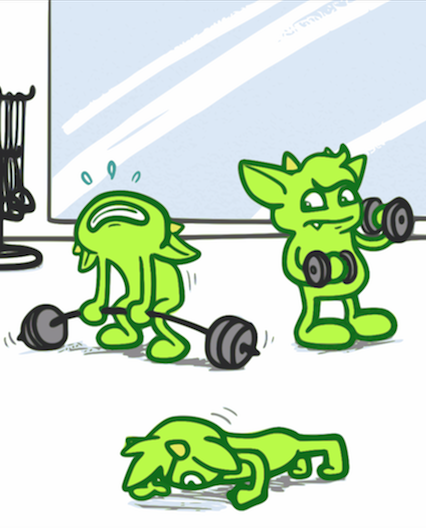
\includegraphics[width=0.7\columnwidth]{img/gremlin-images/gremlin-gym-crop.png}
        \end{column}%
    \end{columns}
    \vfill
    A number of technologies and programming languages had to be learned in order to perform the investigation.
    \vfill
    \parnotes
\end{frame}

%%%%%%%%%%%%%%%%%%%%%%%%%%%%%%%
\section{NoSQL Technology}
%%%%%%%%%%%%%%%%%%%%%%%%%%%%%%%

\begin{frame}{NoSQL Technology}
    In order of least to most structured:
    \vfill
    \begin{tabular}{p{2.4cm}|p{7.5cm}}
        \textbf{Category} & \textbf{Description} \\
        \hline
        \hline
        Key-value store & Keys as identifiers to values as a data object or collection of data objects. \\
        \hline
        Document store & A key-value store but values are document types e.g. JSON, XML. Both keys and values are fully searchable. \\
        \hline
        Column family & Store data along columns as column-families. Column-families are grouped together in keyspaces. \\
        \hline
        Graph & Graph abstraction of storage backend. Backed usually a column-family store or relational database.\\
    \end{tabular}
    \vfill
    NoSQL aims to relax on enforcing \textbf{consistency} and \textbf{structure} to improve \textbf{partition tolerance} and \textbf{availability}.
\end{frame}

%%%%%%%%%%%%%%%%%%%%%%%%%%%%%%%
\section{Graph Query Languages}
%%%%%%%%%%%%%%%%%%%%%%%%%%%%%%%

\begin{frame}{Graph Query Languages}
    The following graph query languages were considered:
    \vfill
    \begin{itemize}
        \item \textbf{Gremlin}: The traversal language of Apache TinkerPop.
        \item \textbf{Cypher}: Graph pattern matching language by Neo4j.
        \item \textbf{GSQL}: TigerGraph's graph query language.
    \end{itemize}
    \vfill
    
\includegraphics[width=.25\textwidth]{img/graph-lang/gremlin-running.png}
    \hfill
    
\includegraphics[width=.25\textwidth]{img/graph-lang/neo4j.png}
    \hfill
    
\includegraphics[width=.25\textwidth]{img/database-logos/tigergraph.png}
\end{frame}

\begin{frame}{Gremlin}
    \begin{columns}
        \begin{column}{.6\textwidth}
            \begin{itemize}
                \item Functional, data-flow query language.
                \item Integrates with multiple vendors e.g. JanusGraph.
                \item Queries can be both imperative or declarative.
                \item Embeds itself into host programming language.
                \item Turing-complete.
            \end{itemize}
            \end{column}%
            \hfill%
            \begin{column}{.39\textwidth}
            \centering
            
\includegraphics[width=0.7\columnwidth]{img/graph-lang/gremlin-running.png}
        \end{column}%
    \end{columns}
\end{frame}

\begin{frame}{Gremlin}
    An example of imperative Gremlin in this project:
    \lstinputlisting[
    language=gremlin,
    caption={
        A Gremlin query that returns recommending users of ``Kate''. These are users who have rated restaurants that Kate has been to above 3 stars.
    },
    label={lst:gremlin1}
    ]
    {./queries/kate.groovy}
\end{frame}

\begin{frame}{Cypher}
    \begin{columns}
        \begin{column}{.6\textwidth}
            \begin{itemize}
                \item Declarative pattern matching query language.
                \item Can compile into other graph query languages e.g. Gremlin, GSQL.
                \item Makes use of ASCII-art in syntax.
                \item SQL-like and aims to be concise and easy to learn.
                \item Not Turing-complete.
            \end{itemize}
            \end{column}%
            \hfill%
            \begin{column}{.39\textwidth}
            \centering
            
\includegraphics[width=0.7\columnwidth]{img/graph-lang/neo4j.png}
        \end{column}%
    \end{columns}
\end{frame}

\begin{frame}{Cypher}
    An example of an application of Cypher on this dataset:
\lstinputlisting[
    language=cypher,
    caption={Returns all users who have reviewed the same businesses as a given user. The query iterates through all users. Note how the return match verifies that the user \texttt{p1} does not match user \texttt{p2}.}
    ]
    {./queries/reviews.cql}
\end{frame}

\begin{frame}{GSQL}
    \begin{columns}
        \begin{column}{.6\textwidth}
            \begin{itemize}
                \item SQL-like language similar to Gremlin and Cypher.
                \item Queries can be both imperative or declarative.
                \item Can accumulate data simultaneously.
                \item Procedural and parameterized queries.
                \item Turing-complete.
            \end{itemize}
            \end{column}%
            \hfill%
            \begin{column}{.39\textwidth}
            \centering
            
\includegraphics[width=0.7\columnwidth]{img/database-logos/tigergraph.png}
        \end{column}%
    \end{columns}
\end{frame}

\begin{frame}{GSQL}
    An example of the GSQL implementation of Listing \ref{lst:gremlin1}.
\lstinputlisting[
    language=gsql,
    caption={A GSQL query that returns recommending users of ``Kate''. These are users who have rated restaurants that Kate has been to above 3 stars.},
    label={lst:gsql1}
    ]
    {./queries/kate1-1.gsql}
\end{frame}

\begin{frame}{GSQL}
    Listing \ref{lst:gsql1} continued.
\lstinputlisting[
    language=gsql,
    caption={A GSQL query that returns recommending users of ``Kate''. These are users who have rated restaurants that Kate has been to above 3 stars.}
    ]
    {./queries/kate1-2.gsql}
\end{frame}

%%%%%%%%%%%%%%%%%%%%%%%%%%%%%%%
\section{Indexing Techniques}
%%%%%%%%%%%%%%%%%%%%%%%%%%%%%%%

\begin{frame}{Indexing Techniques}
    The following types of indexing were used to speed up data retrieval:
    \vfill
    \begin{itemize}
        \item \textbf{B-tree}: Single-dimensional indexing.
        \item \textbf{R-tree}: Multi-dimensional indexing.
        \item \textbf{Geo-grid}: Geohash implementation on a graph.
    \end{itemize}
    \vfill
    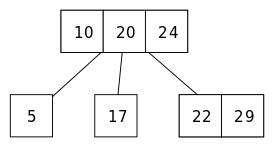
\includegraphics[width=.25\textwidth]{img/index/btree.png}
    \hfill
    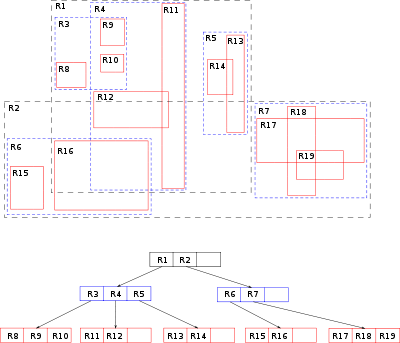
\includegraphics[width=.35\textwidth]{img/index/400px-R-tree.png}
    \hfill
    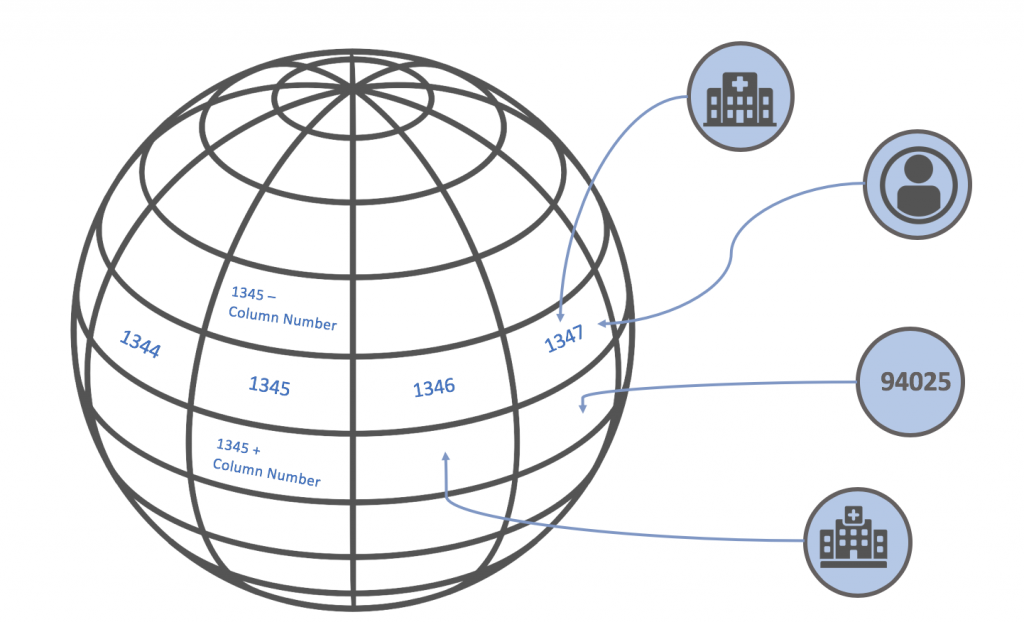
\includegraphics[width=.35\textwidth]{img/index/geogrid.png}
\end{frame}

%%%%%%%%%%%%%%%%%%%%%%%%%%%%%%%
\section{Data Analysis}
%%%%%%%%%%%%%%%%%%%%%%%%%%%%%%%

\begin{frame}{Data Analysis}
    \begin{columns}
        \begin{column}{.7\textwidth}
            \begin{itemize}
                \item Large amounts of \textbf{text data} in dataset from restaurant/business reviews.
                \item \textbf{Sentiment analysis} is performed with NLTK\parnote{The Natural Language Toolkit. Written in Python. \url{www.nltk.org}.} -- extract additional information from review data.
                \item A \textbf{Na\"ive Bayes classifier} used for binary classification.
                \item \textbf{Kernels} represent some ``real-world'' data analysis and associated database operation(s).
                \item Database \textbf{performance} measured during each kernel.
            \end{itemize}
            \end{column}%
            \hfill%
            \begin{column}{.29\textwidth}
            \centering
            
\includegraphics[width=\columnwidth]{img/nltk-logo.png}
        \end{column}%
    \end{columns}
    \vfill
    \parnotes
\end{frame}


%%
% I'm wondering if I should just add a brief hint at this to draw more attention to
% to the demo and further add to the amount of work that was done in this project
%
% Also, front-end/frontend/front end seems be a debate online and change depending
% on how they are used. Compound noun seems to be the best for this instance.
%%
\begin{frame}{Implementation}
    The kernels were implemented in a web application context with the following technologies:
    \vfill
    \begin{itemize}
        \item \textbf{Angular} front-end framework to start kernel jobs and view results.
        \item \textbf{Flask} back-end to schedule jobs, call queries, and perform analysis.
        \item \textbf{Docker} to containerize databases and web application.
    \end{itemize}
    \vfill
    
\includegraphics[width=.25\textwidth]{img/webapp/angular-logo.png}
    \hfill
    
\includegraphics[width=.25\textwidth]{img/webapp/flask-logo.png}
    \hfill
    
\includegraphics[width=.25\textwidth]{img/webapp/docker-whale.png}
\end{frame}

\begin{frame}{Kernel 1: Kate's Restaurant Recommendations}
    \textbf{User story}
    \begin{quote}
        A user, called Kate, would like recommendations for restaurants in an area she does not frequent. Similar users are gathered and restaurants they held in high regard (recently and in that area) are recommended.
    \end{quote}
    \textbf{Query Complexity and Constraints}
    \begin{itemize}
        \item 5 joins
        \item 1-hop -- check that a business belongs to ``Restaurants'' category.
        \item 1 spatial constraint per user -- 5km radius
        \item a \emph{range} and \emph{limit} temporal constraint per user
    \end{itemize}
    
    \medskip
    
    Relative complexity: \textbf{HIGH}
\end{frame}

\begin{frame}{Kernel 2: Phoenix Business Reviews 2018}
    \textbf{User story}
    \begin{quote}
        Characteristics of reviews (per star) are compared for businesses during the 2018 year in the Phoenix area.
    \end{quote}
    \textbf{Query Complexity and Constraints}
    \begin{itemize}
        \item 1 join
        \item 1 spatial query -- 50km radius
        \item 1 \emph{equality} temporal constraint
    \end{itemize}
    
    \medskip
    
    Relative complexity: \textbf{LOW}
\end{frame}

\begin{frame}{Kernel 3: Julie's Holiday Destination Analysis}
    \textbf{User story}
    \begin{quote}
        A user with many friends, called Julie, is going to Las Vegas over the Nov -- Dec period. Instead of asking all her friends for their opinions, the reviews her direct and mutual friends wrote will be used to gauge their opinion of businesses in Las Vegas during the Nov -- Dec period.
    \end{quote}
    \textbf{Query Complexity and Constraints}
    \begin{itemize}
        \item 3 joins
        \item 2-hop -- friends-of-friends query
        \item 1 spatial query -- 30km radius
        \item 1 \emph{range} temporal constraint
    \end{itemize}
    
    \medskip
    
    Relative complexity: \textbf{MEDIUM}
\end{frame}

%%%%%%%%%%%%%%%%%%%%%%%%%%%%%%%
\section{Query Response Times}
%%%%%%%%%%%%%%%%%%%%%%%%%%%%%%%

\begin{frame}{Kernel 1: Response Times}
    TODO: Show graph with increasing data size
\end{frame}

\begin{frame}{Kernel 2: Response Times}
    TODO: Show graph with increasing data size
\end{frame}

\framepic{./img/graphs/kern2.png}

\begin{frame}{Kernel 3: Response Times}
    TODO: Show graph with increasing data size
\end{frame}

\framepic{./img/graphs/cityGraph.png}

%%%%%%%%%%%%%%%%%%%%%%%%%%%%%%%
\section{Conclusion}
%%%%%%%%%%%%%%%%%%%%%%%%%%%%%%%

\begin{frame}{Conclusion}
    This investigation demonstrated that:
    \vfill
    \begin{itemize}
        \item For complex, spatio-temporal queries graph databases are \textbf{superior} to relational databases in terms of query response times
        \item Graph query languages\dots
        \begin{itemize}
            \item aren't necessarily more difficult to learn than SQL
            \item are often \textbf{more concise or expressive} than SQL when writing graph traversals
        \end{itemize}
        \item Data can be \textbf{visualized} as a graph for an additional analysis advantage
        \item Modern graph databases support\dots
        \begin{itemize}
            \item ACID-compliance
            \item web security measures e.g. SSO and LDAP authentication
        \end{itemize}
    \end{itemize}
    \vfill
    Graph databases are \textbf{suitable} for use in the \textbf{analysis of spatio-temporal data} in  enterprise-level applications.
\end{frame}

\begin{frame}{Future Work}
    Add an additional\dots
    \begin{itemize}
        \item spatio-temporal dataset
        \item NewSQL database e.g. MySQL Cluster, Citus for PostgreSQL, etc.
        \item less or more structured NoSQL database e.g. HBase, Facebook's Tao, etc.
        \item search engine e.g. Solr, Lucene, etc.
    \end{itemize}
    \vfill
    Compare server resource consumption \dots
    \begin{itemize}
        \item storage
        \item memory
        \item CPU
    \end{itemize}
\end{frame}

\end{document}
